% This file was converted to LaTeX by Writer2LaTeX ver. 1.0.2
% see http://writer2latex.sourceforge.net for more info
\documentclass[12pt]{article}
\usepackage[utf8]{inputenc}
\usepackage[T1]{fontenc}
\usepackage[english]{babel}
\usepackage{amsmath}
\usepackage{amssymb,amsfonts,textcomp}
\usepackage{array}
\usepackage{supertabular}
\usepackage{hhline}
\usepackage{hyperref}
\hypersetup{colorlinks=true, linkcolor=blue, citecolor=blue, filecolor=blue, urlcolor=blue}
\usepackage{graphicx}
% Text styles
\newcommand\textstyleListLabelxvi[1]{#1}
\makeatletter
\newcommand\arraybslash{\let\\\@arraycr}
\makeatother
\raggedbottom
% Paragraph styles
\renewcommand\familydefault{\rmdefault}
\newenvironment{styleStandard}{\setlength\leftskip{0cm}\setlength\rightskip{0cm plus 1fil}\setlength\parindent{0cm}\setlength\parfillskip{0pt plus 1fil}\setlength\parskip{0in plus 1pt}\writerlistparindent\writerlistleftskip\leavevmode\normalfont\normalsize\writerlistlabel\ignorespaces}{\unskip\vspace{0.111in plus 0.0111in}\par}
\newenvironment{stylelsAbstract}{\setlength\leftskip{0.5in}\setlength\rightskip{0.5in}\setlength\parindent{0in}\setlength\parfillskip{0pt plus 1fil}\setlength\parskip{0in plus 1pt}\writerlistparindent\writerlistleftskip\leavevmode\normalfont\normalsize\itshape\writerlistlabel\ignorespaces}{\unskip\vspace{0.111in plus 0.0111in}\par}
\newenvironment{stylelsSectioni}{\setlength\leftskip{0.25in}\setlength\rightskip{0in plus 1fil}\setlength\parindent{0in}\setlength\parfillskip{0pt plus 1fil}\setlength\parskip{0.1665in plus 0.016649999in}\writerlistparindent\writerlistleftskip\leavevmode\normalfont\normalsize\fontsize{18pt}{21.6pt}\selectfont\bfseries\writerlistlabel\ignorespaces}{\unskip\vspace{0.0835in plus 0.00835in}\par}
\newenvironment{stylelsSectionii}{\setlength\leftskip{0.25in}\setlength\rightskip{0in plus 1fil}\setlength\parindent{0in}\setlength\parfillskip{0pt plus 1fil}\setlength\parskip{0.222in plus 0.0222in}\writerlistparindent\writerlistleftskip\leavevmode\normalfont\normalsize\fontsize{16pt}{19.2pt}\selectfont\bfseries\writerlistlabel\ignorespaces}{\unskip\vspace{0.0835in plus 0.00835in}\par}
\newenvironment{stylelsEnumerated}{\renewcommand\baselinestretch{1.0}\setlength\leftskip{0cm}\setlength\rightskip{0cm plus 1fil}\setlength\parindent{0cm}\setlength\parfillskip{0pt plus 1fil}\setlength\parskip{0in plus 1pt}\writerlistparindent\writerlistleftskip\leavevmode\normalfont\normalsize\writerlistlabel\ignorespaces}{\unskip\vspace{0.0972in plus 0.00972in}\par}
\newenvironment{stylelsBulletList}{\setlength\leftskip{0cm}\setlength\rightskip{0cm plus 1fil}\setlength\parindent{0cm}\setlength\parfillskip{0pt plus 1fil}\setlength\parskip{0cm plus 1pt}\writerlistparindent\writerlistleftskip\leavevmode\normalfont\normalsize\writerlistlabel\ignorespaces}{\unskip\vspace{0cm plus 1pt}\par}
\newenvironment{stylelsLanginfo}{\renewcommand\baselinestretch{1.0}\setlength\leftskip{0.0783in}\setlength\rightskip{0in plus 1fil}\setlength\parindent{0in}\setlength\parfillskip{0pt plus 1fil}\setlength\parskip{0in plus 1pt}\writerlistparindent\writerlistleftskip\leavevmode\normalfont\normalsize\writerlistlabel\ignorespaces}{\unskip\vspace{0in plus 1pt}\par}
% List styles
\newcommand\writerlistleftskip{}
\newcommand\writerlistparindent{}
\newcommand\writerlistlabel{}
\newcommand\writerlistremovelabel{\aftergroup\let\aftergroup\writerlistparindent\aftergroup\relax\aftergroup\let\aftergroup\writerlistlabel\aftergroup\relax}
\newcounter{listWWNumxxiileveli}
\newcounter{listWWNumxxiilevelii}[listWWNumxxiileveli]
\newcounter{listWWNumxxiileveliii}[listWWNumxxiilevelii]
\newcounter{listWWNumxxiileveliv}[listWWNumxxiileveliii]
\renewcommand\thelistWWNumxxiileveli{\arabic{listWWNumxxiileveli}}
\renewcommand\thelistWWNumxxiilevelii{\arabic{listWWNumxxiileveli}.\arabic{listWWNumxxiilevelii}}
\renewcommand\thelistWWNumxxiileveliii{\arabic{listWWNumxxiileveli}.\arabic{listWWNumxxiilevelii}.\arabic{listWWNumxxiileveliii}}
\renewcommand\thelistWWNumxxiileveliv{\arabic{listWWNumxxiileveli}.\arabic{listWWNumxxiilevelii}.\arabic{listWWNumxxiileveliii}.\arabic{listWWNumxxiileveliv}}
\newcommand\labellistWWNumxxiileveli{\thelistWWNumxxiileveli.}
\newcommand\labellistWWNumxxiilevelii{\thelistWWNumxxiilevelii.}
\newcommand\labellistWWNumxxiileveliii{\thelistWWNumxxiileveliii.}
\newcommand\labellistWWNumxxiileveliv{\thelistWWNumxxiileveliv.}
\newenvironment{listWWNumxxiileveli}{\def\writerlistleftskip{\addtolength\leftskip{0.0cm}}\def\writerlistparindent{}\def\writerlistlabel{}\def\item{\def\writerlistparindent{\setlength\parindent{-0cm}}\def\writerlistlabel{\stepcounter{listWWNumxxiileveli}\makebox[0cm][l]{\labellistWWNumxxiileveli}\hspace{0cm}\writerlistremovelabel}}}{}
\newenvironment{listWWNumxxiilevelii}{\def\writerlistleftskip{\addtolength\leftskip{0.0cm}}\def\writerlistparindent{}\def\writerlistlabel{}\def\item{\def\writerlistparindent{\setlength\parindent{-0cm}}\def\writerlistlabel{\stepcounter{listWWNumxxiilevelii}\makebox[0cm][l]{\labellistWWNumxxiilevelii}\hspace{0cm}\writerlistremovelabel}}}{}
\newenvironment{listWWNumxxiileveliii}{\def\writerlistleftskip{\addtolength\leftskip{0.0cm}}\def\writerlistparindent{}\def\writerlistlabel{}\def\item{\def\writerlistparindent{\setlength\parindent{-0cm}}\def\writerlistlabel{\stepcounter{listWWNumxxiileveliii}\makebox[0cm][r]{\labellistWWNumxxiileveliii}\hspace{0cm}\writerlistremovelabel}}}{}
\newenvironment{listWWNumxxiileveliv}{\def\writerlistleftskip{\addtolength\leftskip{0.0cm}}\def\writerlistparindent{}\def\writerlistlabel{}\def\item{\def\writerlistparindent{\setlength\parindent{-0cm}}\def\writerlistlabel{\stepcounter{listWWNumxxiileveliv}\makebox[0cm][l]{\labellistWWNumxxiileveliv}\hspace{0cm}\writerlistremovelabel}}}{}
\newcounter{listWWNumxleveli}
\newcounter{listWWNumxlevelii}[listWWNumxleveli]
\newcounter{listWWNumxleveliii}[listWWNumxlevelii]
\newcounter{listWWNumxleveliv}[listWWNumxleveliii]
\renewcommand\thelistWWNumxleveli{\arabic{listWWNumxleveli}}
\renewcommand\thelistWWNumxlevelii{\alph{listWWNumxlevelii}}
\renewcommand\thelistWWNumxleveliii{\roman{listWWNumxleveliii}}
\renewcommand\thelistWWNumxleveliv{\arabic{listWWNumxleveliv}}
\newcommand\labellistWWNumxleveli{\thelistWWNumxleveli.}
\newcommand\labellistWWNumxlevelii{\thelistWWNumxlevelii.}
\newcommand\labellistWWNumxleveliii{\thelistWWNumxleveliii.}
\newcommand\labellistWWNumxleveliv{\thelistWWNumxleveliv.}
\newenvironment{listWWNumxleveli}{\def\writerlistleftskip{\addtolength\leftskip{0.0cm}}\def\writerlistparindent{}\def\writerlistlabel{}\def\item{\def\writerlistparindent{\setlength\parindent{-0cm}}\def\writerlistlabel{\stepcounter{listWWNumxleveli}\makebox[0cm][l]{\labellistWWNumxleveli}\hspace{0cm}\writerlistremovelabel}}}{}
\newenvironment{listWWNumxlevelii}{\def\writerlistleftskip{\addtolength\leftskip{0.0cm}}\def\writerlistparindent{}\def\writerlistlabel{}\def\item{\def\writerlistparindent{\setlength\parindent{-0cm}}\def\writerlistlabel{\stepcounter{listWWNumxlevelii}\makebox[0cm][l]{\labellistWWNumxlevelii}\hspace{0cm}\writerlistremovelabel}}}{}
\newenvironment{listWWNumxleveliii}{\def\writerlistleftskip{\addtolength\leftskip{0.0cm}}\def\writerlistparindent{}\def\writerlistlabel{}\def\item{\def\writerlistparindent{\setlength\parindent{-0cm}}\def\writerlistlabel{\stepcounter{listWWNumxleveliii}\makebox[0cm][r]{\labellistWWNumxleveliii}\hspace{0cm}\writerlistremovelabel}}}{}
\newenvironment{listWWNumxleveliv}{\def\writerlistleftskip{\addtolength\leftskip{0.0cm}}\def\writerlistparindent{}\def\writerlistlabel{}\def\item{\def\writerlistparindent{\setlength\parindent{-0cm}}\def\writerlistlabel{\stepcounter{listWWNumxleveliv}\makebox[0cm][l]{\labellistWWNumxleveliv}\hspace{0cm}\writerlistremovelabel}}}{}
\newcommand\labellistWWNumixleveli{[F0B7?]}
\newcommand\labellistWWNumixlevelii{\textstyleListLabelxvi{o}}
\newcommand\labellistWWNumixleveliii{[F0A7?]}
\newcommand\labellistWWNumixleveliv{[F0B7?]}
\newenvironment{listWWNumixleveli}{\def\writerlistleftskip{\addtolength\leftskip{0.0cm}}\def\writerlistparindent{}\def\writerlistlabel{}\def\item{\def\writerlistparindent{\setlength\parindent{-0cm}}\def\writerlistlabel{\makebox[0cm][l]{\labellistWWNumixleveli}\hspace{0cm}\writerlistremovelabel}}}{}
\newenvironment{listWWNumixlevelii}{\def\writerlistleftskip{\addtolength\leftskip{0.0cm}}\def\writerlistparindent{}\def\writerlistlabel{}\def\item{\def\writerlistparindent{\setlength\parindent{-0cm}}\def\writerlistlabel{\makebox[0cm][l]{\labellistWWNumixlevelii}\hspace{0cm}\writerlistremovelabel}}}{}
\newenvironment{listWWNumixleveliii}{\def\writerlistleftskip{\addtolength\leftskip{0.0cm}}\def\writerlistparindent{}\def\writerlistlabel{}\def\item{\def\writerlistparindent{\setlength\parindent{-0cm}}\def\writerlistlabel{\makebox[0cm][l]{\labellistWWNumixleveliii}\hspace{0cm}\writerlistremovelabel}}}{}
\newenvironment{listWWNumixleveliv}{\def\writerlistleftskip{\addtolength\leftskip{0.0cm}}\def\writerlistparindent{}\def\writerlistlabel{}\def\item{\def\writerlistparindent{\setlength\parindent{-0cm}}\def\writerlistlabel{\makebox[0cm][l]{\labellistWWNumixleveliv}\hspace{0cm}\writerlistremovelabel}}}{}
\newcounter{listWWNumiileveli}
\newcounter{listWWNumiilevelii}[listWWNumiileveli]
\newcounter{listWWNumiileveliii}[listWWNumiilevelii]
\newcounter{listWWNumiileveliv}[listWWNumiileveliii]
\renewcommand\thelistWWNumiileveli{\arabic{listWWNumiileveli}}
\renewcommand\thelistWWNumiilevelii{\alph{listWWNumiilevelii}}
\renewcommand\thelistWWNumiileveliii{}
\renewcommand\thelistWWNumiileveliv{}
\newcommand\labellistWWNumiileveli{(\thelistWWNumiileveli)}
\newcommand\labellistWWNumiilevelii{\thelistWWNumiilevelii.}
\newcommand\labellistWWNumiileveliii{\thelistWWNumiileveliii}
\newcommand\labellistWWNumiileveliv{\thelistWWNumiileveliv}
\newenvironment{listWWNumiileveli}{\def\writerlistleftskip{\addtolength\leftskip{0.0cm}}\def\writerlistparindent{}\def\writerlistlabel{}\def\item{\def\writerlistparindent{\setlength\parindent{-0cm}}\def\writerlistlabel{\stepcounter{listWWNumiileveli}\makebox[0cm][l]{\labellistWWNumiileveli}\hspace{0cm}\writerlistremovelabel}}}{}
\newenvironment{listWWNumiilevelii}{\def\writerlistleftskip{\addtolength\leftskip{0.0cm}}\def\writerlistparindent{}\def\writerlistlabel{}\def\item{\def\writerlistparindent{\setlength\parindent{-0cm}}\def\writerlistlabel{\stepcounter{listWWNumiilevelii}\makebox[0cm][l]{\labellistWWNumiilevelii}\hspace{0cm}\writerlistremovelabel}}}{}
\newenvironment{listWWNumiileveliii}{\def\writerlistleftskip{\addtolength\leftskip{0.0cm}}\def\writerlistparindent{}\def\writerlistlabel{}\def\item{\def\writerlistparindent{\setlength\parindent{-0cm}}\def\writerlistlabel{\stepcounter{listWWNumiileveliii}\makebox[0cm][l]{\labellistWWNumiileveliii}\hspace{0cm}\writerlistremovelabel}}}{}
\newenvironment{listWWNumiileveliv}{\def\writerlistleftskip{\addtolength\leftskip{0.0cm}}\def\writerlistparindent{}\def\writerlistlabel{}\def\item{\def\writerlistparindent{\setlength\parindent{-0cm}}\def\writerlistlabel{\stepcounter{listWWNumiileveliv}\makebox[0cm][l]{\labellistWWNumiileveliv}\hspace{0cm}\writerlistremovelabel}}}{}
\setlength\tabcolsep{1mm}
\renewcommand\arraystretch{1.3}
% footnotes configuration
\makeatletter
\renewcommand\thefootnote{\arabic{footnote}}
\makeatother
\title{}
\author{UIC}
\date{2018-01-17}
\begin{document}
\title{\textsuperscript{Assessing} learners’ changes in foreign accent during Study Abroad}
\maketitle

\begin{styleStandard}
\textit{Pilar Avello, Universidad Pompeu Fabra}
\end{styleStandard}

\begin{stylelsAbstract}
The present study aims to contribute to the field of Study Abroad (SA) research by exploring the under-investigated interface between SA and the measurement of pronunciation gains in terms of improvement in degree of foreign accent (FA). It is an exploratory study which analyzes changes in FA measures as a result of a short-term, 3-month SA program preceded by a Formal Instruction (FI) period. Data were collected from a group of non-native speakers (NNSs) consisting of 8 undergraduate, upper-intermediate learners of English as a second language (L2) with Catalan and Spanish as first languages (L1s), and from 3 undergraduate L1 English native speakers (NSs), who served as controls. Data from the NNSs were collected at the beginning of their degree (T1), after an 80-hour FI period (T2), and upon their return from SA (T3); data from the NSs were collected only once (T0). Thirteen L1 English listeners rated the speech samples from the NSs and the NNS for degree of FA by means of a rating experiment using a Likert scale. Analyses failed to yield a significant effect of SA on FA ratings and did not reveal a significant difference in FA ratings following SA as compared to FI. These findings are in line with the inconclusive and mixed results which are often reported for L2 pronunciation in short-term SA contexts.
\end{stylelsAbstract}

\setcounter{listWWNumxxiileveli}{0}
\begin{listWWNumxxiileveli}
\item 
\begin{stylelsSectioni}
Introduction
\end{stylelsSectioni}

\end{listWWNumxxiileveli}
\begin{styleStandard}
Over the last decades, Study Abroad (SA) programs have enjoyed increasing popularity worldwide, particularly at university level. The ever-growing popularity of SA is arguably linked to the widespread belief that an overseas program has substantial linguistic benefits for students. This belief is based on the assumption that immersion in the target language community is the best way to acquire the language due to the opportunities for interaction and the amount and quality of the input available in this learning context.
\end{styleStandard}

\begin{styleStandard}
Academic authorities and governments have played an active role in the promotion of SA programs, encouraging students to go abroad so as to improve their second language (L2) proficiency. One of the most popular examples is the inter-university Erasmus program in the European Union. Hundreds of thousands of students from the different European countries have received an Erasmus grant in order to pursue part of their university studies in a different European country, and Spain, where the present study has been conducted, is one of the countries which have benefited the most from this program, both in terms of outgoing and incoming students.
\end{styleStandard}

\begin{styleStandard}
In this scenario, the need to empirically assess the actual benefits of SA on learners’ L2 development has become evident. A growing body of research within the field of L2 acquisition has been devoted to this learning context in order to analyze the effects of SA on the different linguistic skills. Contributions to this body of research within a European perspective have been particularly called for, given the fact that an important part of SA research has been conducted from a North American perspective (Coleman 1998). 
\end{styleStandard}

\begin{styleStandard}
An overview of the existing SA literature does not indicate substantial SA gains for all the different linguistic skills across the board (cf. DeKeyser 2007). Results point to clear benefits in areas such as vocabulary growth, socio-pragmatic skills and overall oral proficiency, and especially regarding fluency, which has been one of the most extensively researched areas. However, the domain of phonology, which is the focus of the present study, has been the object of relatively little research within the SA literature, and findings so far are inconclusive as to the changes that can accrue in L2 speech perception and production during a period abroad. This is particularly remarkable, considering that one of the main aims of students going abroad is to improve their L2 pronunciation, which is normally far from native norms in the case of learners who have been exposed to foreign-accented input in formal instruction (FI) settings. 
\end{styleStandard}

\begin{styleStandard}
Research into L2 phonological acquisition in contexts of naturalistic, long-term immersion has shown that pronunciation is one area of L2 proficiency particularly resistant to change, even in an environment of massive and authentic L2 input exposure. Learners’ difficulties in achieving native pronunciation norms are evidenced by a perceptible foreign accent, which is largely the reflection of the learners’ first language (L1) phonology. In fact, research into L2 phonological acquisition, which has usually adopted a cross-sectional design, has established that one of the main causes underlying learners’ difficulties in acquiring a new L2 phonology is the influence of the already existing L1 phonological system (Flege 1995; Best \& Tyler 2007).
\end{styleStandard}

\begin{styleStandard}
Given that the domain of L2 phonology within the SA literature remains under-investigated, we seek to further our understanding of the benefits that can be expected to accrue in this domain during a period abroad. We present the results of a longitudinal, pre-test/post-test design, which assesses the effects of a 3-month SA period preceded by an FI period on a group of L1 Spanish/Catalan undergraduate learners of L2 English.
\end{styleStandard}

\begin{listWWNumxxiileveli}
\item 
\begin{stylelsSectioni}
Literature Review
\end{stylelsSectioni}


\setcounter{listWWNumxxiilevelii}{0}
\begin{listWWNumxxiilevelii}
\item 
\begin{stylelsSectionii}
L2 Speech Development \& Foreign Accent
\end{stylelsSectionii}

\end{listWWNumxxiilevelii}
\end{listWWNumxxiileveli}
\begin{styleStandard}
An important body of research in the field of L2 speech learning has been devoted to examining the phenomenon of foreign accent (FA), also referred to as accentedness in the literature. FA has been described, for instance, as “the extent to which an L2 learner’s speech is perceived to differ from native speaker (NS) norms” (Munro \& Derwing 1998: 160). It has also been characterized as “non-pathological speech produced by second language learners which differs in partially systematic ways from the speech characteristic of native speakers of a given dialect” (Munro 1998: 139). In his seminal work providing a full account of his Speech Learning Model for L2 phonological acquisition, Flege (1995: 233) noted that “[l]isteners hear foreign accents when they detect divergences from English phonetic norms along a wide range of segmental and suprasegmental (i.e., prosodic) dimensions”. 
\end{styleStandard}

\begin{styleStandard}
FA is therefore a perceptual phenomenon related to the processing of L2 speech which results from listeners’ perception of differences between specific properties of L2 speech and those that characterize native speakers’ (NSs) norms. As such, a foreign accent is the perceptual correlate of objective acoustic-phonetic characteristics of L2 learners’ pronunciation which, as pointed out by Flege (1995), can take place both at the segmental level (divergences from the range of native-like acoustic values, or number and severity of pronunciation errors), and at the suprasegmental level (stress, rhythm and intonation patterns which are found to differ from native norms).
\end{styleStandard}

\begin{styleStandard}
Interest in the study of FA within L2 phonological acquisition research arises from its theoretical relevance regarding general theories of L2 acquisition and from its pragmatic dimension related to L2 teaching. From a theoretical perspective, research into the phenomenon of FA may shed light on the existence of age-related constraints that might influence L2 acquisition, as the domain of pronunciation very often evidences incomplete acquisition in adult and adolescent L2 learners. In this line of research, the study of FA has been strongly connected to what some authors have hypothesized as a ‘critical’ or ‘sensitive’ period for L2 acquisition (Lenneberg 1967; Scovel 1988; Long 1990). These authors posit biological and maturational constraints on L2 acquisition that would prevent native-like L2 phonological performance beyond the hypothesized critical or sensitive period, which is generally considered to end around puberty, leading to the emergence of a clearly perceptible foreign accent as a characteristic of L2 learner’s speech.
\end{styleStandard}

\begin{styleStandard}
From a pragmatic perspective, a better understanding of which specific features of L2 speech contribute more to a foreign accent may inform more efficient approaches in the teaching of L2 pronunciation (cf., for instance, Piske, MacKay \& Flege 2001). In this sense, the study of FA has usually been related to research on other dimensions of L2 speech, such as speaking rate (Munro \& Derwing 1998) and fluency, comprehensibility and intelligibility (Munro \& Derwing 1995; Derwing \& Munro 1997; 2013). The aim of these studies is to clarify the interaction between these different speech dimensions and how they affect listeners’ processing of L2 speech, in order to shed light on the best teaching strategies that would facilitate the development of L2 learners’ fluent and successful communication in the L2, which is usually the ultimate goal of the language learner in a context of immersion in the target language community. 
\end{styleStandard}

\begin{styleStandard}
Research in the field of FA has usually adopted the form of experimental studies with a cross-sectional design in which oral data are elicited at a single point in time. Many of these studies focus on immersion contexts in which the target language has been acquired usually without FI (e.g. immigrants from different backgrounds in an English-speaking country like the United States or Canada). Measures of FA are typically obtained by having a group of listeners rate L1 and L2 speech samples for degree of accentedness by means of Likert-type, equal-appearing interval scales. Most studies have analyzed the perception of accentedness by native listeners (NLs), who have been found to provide reliable FA ratings, although non-native listeners have also been found to assess accentedness reliably regardless of whether they share the same L1 with learners. Common data elicitation techniques include having the L2 learners read words, sentences or paragraphs aloud. Sometimes they may be asked to repeat a speech stimulus that has been produced by NSs. Samples of free or extemporaneous speech may also be obtained, for example, by asking the learners to describe a picture or tell a story. 
\end{styleStandard}

\begin{styleStandard}
Age of onset of learning (AOL), identified as age of first exposure to the L2, has been the most examined factor in the FA literature. Interest in the study of age effects on L2 pronunciation is related to the hypothesized critical or sensitive period for language acquisition (Lenneberg 1967; Scovel 1988). However, results from some studies have shown that adult learners may indeed be able to acquire native-like pronunciation (Bongaerts, Planken \& Schils 1995; Flege et al. 1995; Bongaerts, van Summeren, Planken \& Schils 1997). Conversely, some studies have also shown that an early age of L2 acquisition (as early as 3.2 years) does not guarantee accent-free pronunciation (Flege, Frieda \& Nozawa 1997). Many studies have revealed a gradual increase in FA as AOL increases (Flege 1988; Flege \& Fletcher 1992), a finding which points toward a linear relationship between AOL and degree of FA. In general, most research indicates that ‘the earlier the better’ for L2 pronunciation, but it seems that early L2 acquisition is not enough for mastery of the L2. This has led authors to assess the influence of other factors on degree of FA, most notably L2 experience, amount and quality of L2 input, or patterns of L1/L2 use (cf. Piske et al. 2001 for a review). 
\end{styleStandard}

\begin{styleStandard}
L2 experience has been the second most studied factor considered to influence degree of FA. Since most FA studies have been conducted in immersion contexts, L2 experience has been typically operationalized as length of residence (LOR) in the L2 country. Research assessing the effect of LOR on L2 pronunciation has yielded mixed results. Flege \& Fletcher (1992) found that LOR had a significant correlation with FA, as did English-language instruction and AOL. An LOR effect has been usually found for early L2 learners, that is, learners who first encountered massive L2 exposure before the end of the hypothesized critical period (around puberty), whereas increased LOR does not seem to have an impact on late or adult L2 learners following an initial phase of improvement that takes place at the early stage of L2 learning (Flege 1988). Other studies suggest that LOR effects depend on learners’ stage of L2 acquisition (Riney \& Flege 1998; Meador, Flege, Mackay 2000).
\end{styleStandard}

\begin{styleStandard}
Several studies have found that amount and quality of L2 input and language use patterns are also influential factors on L2 pronunciation (Flege et al. 1995; Flege et al., 1997; Piske et al. 2001). These studies make use of self-assessment questionnaires in which learners have to estimate, for instance, the amount of contact with NSs of the L2, the amount of time they spend using their L1 and L2 in different contexts, or L1 and L2 proficiency. Results in Flege et al. (1995) revealed that language use patterns constituted a significant predictor of FA ratings for Italian learners of L2 English, explaining 15\% of the total variance. In a follow-up study (Flege et al. 1997), the role of L1 use was further explored by creating two groups of early Italian/English bilinguals who were AOL-matched (around 6 years old), but who differed in percentage of L1 use (3\% vs. 36\%). The authors reported an L1 use effect as the learners with higher L1 use were perceived to have a significantly stronger FA than the learners with lower L1 use. Results in Piske et al. (2001) showed that the L1 use effect observed for early bilinguals was also extended to late Italian/English bilinguals.
\end{styleStandard}

\begin{styleStandard}
Results from these studies indicate that, although AOL has been found to be the most influential factor in the development of L2 pronunciation, differences in L2 pronunciation outcomes can also be the result of the interplay of other factors such as the amount and quality of the L2 input to which learners are exposed, as well as patterns of L1/L2 language use. However, as already noted, studies examining the phenomenon of FA have been mainly conducted in contexts of long-term immersion, rather than in shorter periods of immersion, such as those typical of SA learning contexts.
\end{styleStandard}

\begin{listWWNumxxiileveli}
\item 
\setcounter{listWWNumxxiilevelii}{0}
\begin{listWWNumxxiilevelii}
\item 
\begin{stylelsSectionii}
Study Abroad
\end{stylelsSectionii}

\end{listWWNumxxiilevelii}
\end{listWWNumxxiileveli}
\begin{styleStandard}
SA is a context of L2 acquisition characterized by a combination of language-based and/or content-based classroom instruction together with out-of-class interaction in the native speech community (Freed 1995a: 5). SA programs have become very popular in Europe and North America due to the common sense and long-held assumption that immersion in the L2 community results in substantially enhanced L2 knowledge, as such immersion is assumed to offer plenty of opportunities for interaction with NSs and exposure to a great amount of high quality input. Consequently, SA programs have been encouraged by language instructors and academic administrators, and have come to play an important role in governments’ L2 learning policies as a means to promote multilingualism in response to an increasingly globalized international context (cf. Kinginger 2009). A growing body of research has been therefore devoted to this learning context in order to account for the nature of the SA experience and empirically assess its impact on L2 learners’ linguistic development (cf. overviews in Freed 1995a; DuFon \& Churchill 2006). 
\end{styleStandard}

\begin{styleStandard}
For the most part, research has found evidence for a positive effect of the SA experience on learners’ L2 development, yet actual linguistic gains appear to be related to individual and context variables such as contact patterns while abroad, L1 and L2 use, L2 exposure, initial level of L2 proficiency, and length of stay (LoS, operationalized as duration of the SA period), as well as to aspects of program design (see Pérez-Vidal \& Juan-Garau 2011 for a characterization of SA). A complex picture results from the interaction of all these factors, with findings sometimes providing inconclusive or conflicting evidence, as the benefits of SA are not always clear for all language skills, or the gains reported may fall short of the high expectations arising out of the above-mentioned widespread belief in the substantial effects of SA immersion.
\end{styleStandard}

\begin{styleStandard}
Research has analyzed the impact of SA on different linguistic domains, and usually in contrast with FI in at-home (AH) institutions. Results have provided consistent evidence of the beneficial effect of SA for lexical improvement (Collentine 2004; Llanes \& Muñoz 2009), as well as for writing (Sasaki 2004; Pérez-Vidal \& Juan-Garau 2011) and listening (Allen \& Herron 2003; Llanes \& Muñoz 2009). Sociolinguistic skills have been the object of considerable research with studies examining, for instance, communication strategies (Lafford 1995) and pragmatic competence (Barron 2006), which have also yielded results supporting the positive effect of SA on these areas. However, mixed results have been found for grammar; results reported by Collentine (2004) showed more grammatical improvement for AH learners as compared with those who went abroad, whereas the opposite was true in Howard (2005). Most SA research has focused on the development of oral skills, which has traditionally been considered the most likely linguistic domain to improve as a result of SA, and research findings in general have supported this view. Some studies have analyzed the impact of SA on overall L2 speaking proficiency (Brecht, Davidson \& Ginsberg 1995; Segalowitz \& Freed 2004), and extensive research has also been carried out to analyze gains in L2 learners’ fluency (Freed 1995b; Freed, Dewey, Segalowitz \& Halter 2004, Valls-Ferrer 2011). 
\end{styleStandard}

\begin{styleStandard}
However, studies focusing on specific aspects of phonological development in learners’ L2 speech production during SA are scarce. The few existing studies generally focus on the differential effects of SA versus FI on L2 pronunciation, and have yielded mixed results. Díaz-Campos (2004) reported a positive effect of both learning contexts on the production of Spanish plosives in two groups of English students of Spanish, although development toward native-like patterns was found to be stronger in the FI group. In contrast, Díaz-Campos (2006) observed greater gains in the production of Spanish consonants for the SA group as compared with the FI group. Mora (2008) examined the production of voice onset time in English voiceless plosives by a group of L1 Spanish/Catalan bilingual learners after a two-term FI period at their home university and after a 3-month SA term abroad. He found no effect of FI on voice onset time duration, whereas a non-significant increase was observed after SA. However, in a study with a similar population analyzing English vowels, significant improvement in production was found after FI, but not after SA (Pérez-Vidal, Juan-Garau \& Mora 2011). Sanz, Morales-Front, Nagle \& Moorman (2013) reported significant SA gains in the production of L2 plosives by L1 English learners of Spanish, whereas Simões (1996) did not find significant improvement in the production of Spanish vowels for L1 English learners following SA. Del Río (2013) found significantly greater improvement in FA ratings after SA than FI in a group of adolescent L2 English learners. Højen (2003) found better FA scores after SA as a function of LoS (average = 7.1 months), but production at the segmental level for both vowel and segmental contrasts did not improve significantly. Avello (2010a) also failed to find improvement in the production of vowel contrasts following SA, although in Avello (2010b) the lack of improvement in vowel contrast production did not prevent considerable gains in FA scores. In contrast, Avello, Mora \& Pérez-Vidal (2012) reported significant gains in segmental production in terms of a reduction in error rate scores, but which were not accompanied by significant gains in FA scores.
\end{styleStandard}

\begin{styleStandard}
The present study thus explores the under-investigated impact of SA on L2 learners’ pronunciation development. It is an exploratory study which aims to analyze the interface between SA and FA by assessing the impact of a 3-month SA program on L2 speech production by a group bilingual L1 Catalan/Spanish learners of L2 English by means of FA measures.
\end{styleStandard}

\begin{listWWNumxxiileveli}
\item 
\begin{stylelsSectioni}
Research Aims
\end{stylelsSectioni}

\end{listWWNumxxiileveli}
\setcounter{listWWNumxleveli}{0}
\begin{listWWNumxleveli}
\item 
\begin{stylelsEnumerated}
To assess possible differential effects of type of instruction through time on global FA ratings by analyzing the impact of a 3-month SA period preceded by an 80-hour FI learning context.
\end{stylelsEnumerated}

\item 
\begin{stylelsEnumerated}
To assess differences between native and non-native FA ratings and whether a development through time toward native norms can be observed in L2 learners’ FA ratings as a function of learning context.
\end{stylelsEnumerated}

\end{listWWNumxleveli}
\setcounter{listWWNumxxiileveli}{0}
\begin{listWWNumxxiileveli}
\item 
\begin{stylelsSectioni}
Method
\end{stylelsSectioni}


\setcounter{listWWNumxxiilevelii}{0}
\begin{listWWNumxxiilevelii}
\item 
\begin{stylelsSectionii}
Design
\end{stylelsSectionii}

\end{listWWNumxxiilevelii}
\end{listWWNumxxiileveli}
\begin{styleStandard}
The data presented in this paper are part of the Study Abroad and Language Acquisition (SALA) project. This is a large, state-funded project based at a University in Barcelona, Spain, which analyzes the development of linguistic proficiency in upper-intermediate learners of L2 English who experience an SA period preceded by an FI period (see full description in Pérez-Vidal \& Juan-Garau 2011). This project has a longitudinal, pre-test/post-test design in order to assess possible differential effects of the FI period at the AH university versus the subsequent short-term SA period on the learners’ L2 linguistic development. Data were collected at three different points in time covering a 15-month period:
\end{styleStandard}

\begin{listWWNumixleveli}
\item 
\begin{stylelsBulletList}
T1: at the beginning of the first academic year, to assess initial L2 proficiency.
\end{stylelsBulletList}

\item 
\begin{stylelsBulletList}
T2: after an 80-hour FI period, to assess the impact of this classroom learning context on the learners’ L2 proficiency. Exposure to English in this learning context was basically limited to classroom language learning and was form-focused. The amount of input and communicative interaction was therefore rather limited. Students received no specific phonological training or pronunciation instruction.
\end{stylelsBulletList}

\item 
\begin{stylelsBulletList}
T3: after a compulsory 3-month SA period in an English-speaking country at the beginning of the second academic year, to assess the impact of the SA learning context on the learners’ L2 development. In this context students were expected to receive a massive amount of out-of-class input and to benefit from opportunities for communicative interaction in real, everyday social situations.
\end{stylelsBulletList}

\end{listWWNumixleveli}
\setcounter{listWWNumxxiileveli}{0}
\begin{listWWNumxxiileveli}
\item 
\setcounter{listWWNumxxiilevelii}{0}
\begin{listWWNumxxiilevelii}
\item 
\begin{stylelsSectionii}
Participants
\end{stylelsSectionii}

\end{listWWNumxxiilevelii}
\end{listWWNumxxiileveli}
\begin{styleStandard}
Data were collected from a group of non-native speakers (NNSs, \textit{n} = 8). They shared a similar AOL in AH institutions (AOL = 8 years), as established by the Spanish educational system. Their acquisition of English took place basically through classroom instruction (i.e., as a foreign language in their native speech community), with 700-800 hours of exposure to English. These learners had to certify an upper-intermediate English proficiency level (equivalent to a B2 in the Common European Framework of Reference, or CEFR) in order to be admitted into the AH university.
\end{styleStandard}

\begin{styleStandard}
Speech samples from 3 NSs of American English served as baseline data to assess the learners’ performance. These NSs were young university students enrolled in an L2 Spanish exchange program in Spain. Both groups of speakers had, therefore, a similar profile, and consequently their data were highly comparable. Data from the NSs was collected only once (T0).
\end{styleStandard}

\begin{styleStandard}
A group of English NLs (\textit{n} = 13) were recruited to assess the speech samples from the native and non-native groups for degree of FA; 6 of them were exchange students at a university in Spain and 7 were English teachers.
\end{styleStandard}

\begin{listWWNumxxiileveli}
\item 
\setcounter{listWWNumxxiilevelii}{0}
\begin{listWWNumxxiilevelii}
\item 
\begin{stylelsSectionii}
Speech Samples
\end{stylelsSectionii}

\end{listWWNumxxiilevelii}
\end{listWWNumxxiileveli}
\begin{styleStandard}
Speech samples from the NSs and the NNSs were elicited by means of a reading aloud task, which consisted of the rendition by the participants of the text “The North Wind and the Sun”. The International Phonetic Association (IPA) has encouraged the use of this short, 114-word text as a standard oral elicitation resource to document the pronunciation of different languages and language varieties (cf. IPA 1999), and it has been used to document differences characterizing English pronunciation in different dialects and by L2 learners (see Schneider et al. 2004). 
\end{styleStandard}

\begin{styleStandard}
A member of the research team was present during the recordings to give instructions to the participants on how to perform the reading aloud task and to answer possible questions. Instructions were also provided on the test handout, which participants were asked to read carefully. Participants were recorded individually. They were instructed to read the text twice, first silently on their own in order to become familiar with it, and then out loud to be recorded. The researcher told them that they would be asked a question about the text after reading it the second time. This was done to draw the participants’ attention to the content with the aim of obtaining more natural-sounding data. Immediately after reading the text aloud, they were asked the following question: “Was the North Wind Stronger than the sun?”, which they had to answer by merely stating “yes” or “no”.
\end{styleStandard}

\begin{styleStandard}
Data from the NNSs were recorded in sound-attenuated cabins using an analog tape recorder and were subsequently digitized in .wav format at 22,050, 16 bit monaural. Data from the NSs were recorded in sound-proof cabins using the Pro Tools digital audio workstation platform for Microsoft Windows. The digital files were saved in .wav format at 44,100 Hz (later downsampled to 22,050 Hz), 16 bit monaural.
\end{styleStandard}

\begin{styleStandard}
A sentence extracted from the reading aloud task was used to create the stimuli for the rating task (see §4.4. below).\footnote{ \textit{Then the sun shone out warmly, and immediately the traveler took off his cloak.}} This sentence presented several segmental and suprasegmental properties that were likely to cause the L2 learners to produce pronunciation errors leading to accented L2 production. Some examples of such pronunciation errors as produced by the NNSs are provided in (1-4): 
\end{styleStandard}

\setcounter{listWWNumiileveli}{0}
\begin{listWWNumiileveli}
\item 
\begin{stylelsLanginfo}
Deletions 
\end{stylelsLanginfo}


\setcounter{listWWNumiilevelii}{0}
\begin{listWWNumiilevelii}
\item 
\begin{stylelsLanginfo}
deletion of [l] in \textit{warm(l)y}
\end{stylelsLanginfo}

\item 
\begin{stylelsLanginfo}
deletion of final syllable in \textit{travel(er)}
\end{stylelsLanginfo}

\end{listWWNumiilevelii}
\item 
\begin{stylelsLanginfo}
Insertions
\end{stylelsLanginfo}


\setcounter{listWWNumiilevelii}{0}
\begin{listWWNumiilevelii}
\item 
\begin{stylelsLanginfo}
insertion of an extra vowel [e] in \textit{immediat[e]ly}
\end{stylelsLanginfo}

\item 
\begin{stylelsLanginfo}
insertion of a velar consonant at the beginning of \textit{[[263?]]warmly}
\end{stylelsLanginfo}

\end{listWWNumiilevelii}
\item 
\begin{stylelsLanginfo}
Substitutions
\end{stylelsLanginfo}


\setcounter{listWWNumiilevelii}{0}
\begin{listWWNumiilevelii}
\item 
\begin{stylelsLanginfo}
substitution of bilabial approximant [$\beta $] for velar fricative [v] in \textit{traveler}
\end{stylelsLanginfo}

\item 
\begin{stylelsLanginfo}
substitution of dental plosive [d] for dental fricative [ð] in \textit{then}
\end{stylelsLanginfo}

\item 
\begin{stylelsLanginfo}
substitution of open vowel [a] for close back vowel [[254?]] in \textit{warmly}
\end{stylelsLanginfo}

\item 
\begin{stylelsLanginfo}
substitution of dental fricative [ð] for alveolar plosive [d] in \textit{immediately}
\end{stylelsLanginfo}

\item 
\begin{stylelsLanginfo}
substitution of velar fricative [x] for glottal fricative [h] in \textit{his}
\end{stylelsLanginfo}

\end{listWWNumiilevelii}
\item 
\begin{stylelsLanginfo}
Stress misplacement
\end{stylelsLanginfo}


\setcounter{listWWNumiilevelii}{0}
\begin{listWWNumiilevelii}
\item 
\begin{stylelsLanginfo}
stress shift to the penultimate syllable in multisyllabic words: \textit{tra[2C8?]veler} for \textit{[2C8?]traveler}, \textit{imme[2C8?]diately} for\textit{ i[2C8?]mmediately}.
\end{stylelsLanginfo}

\end{listWWNumiilevelii}
\end{listWWNumiileveli}
\setcounter{listWWNumxxiileveli}{0}
\begin{listWWNumxxiileveli}
\item 
\setcounter{listWWNumxxiilevelii}{0}
\begin{listWWNumxxiilevelii}
\item 
\begin{stylelsSectionii}
Rating Task
\end{stylelsSectionii}

\end{listWWNumxxiilevelii}
\end{listWWNumxxiileveli}
\begin{styleStandard}
A rating task was conducted in order to obtain measures of changes in the learners’ degree of FA through time. This experiment provided us with listeners’ behavioral measures of global FA ratings regarding overall changes in the NNSs’ pronunciation as a result of FI and SA. As noted in §2.1 above, this methodology has been widely used in research on L2 speech production analyzing the construct of FA, as well as other dimensions of L2 speech such as intelligibility and comprehensibility.
\end{styleStandard}

\begin{styleStandard}
The task was a self-paced task created and run with Praat software (Boersma \& Weenink 2008, version 5.1) and displayed on PCs running Microsoft Windows XP OS. Stimuli consisted of speech samples extracted from the reading aloud task as produced by the 3 NSs (T0) and the 8 NNSs (T1, T2 and at T3). The resulting audio files were edited and saved in .wav format at 22,050 Hz, 16 bit monaural, and normalized for intensity at 70.0 dB.
\end{styleStandard}

\begin{styleStandard}
At the beginning of the session, the NLs were given a handout with the description of the experiment, as well as with some instructions on how to run it with Praat. They rated the degree of FA in the oral samples by means of a 5-point equal-appearing Likert scale, where 1 = “native” and 5 = “heavy foreign accent” (see Figure 1 below). 
\end{styleStandard}

\begin{styleStandard}
  [Warning: Image ignored] % Unhandled or unsupported graphics:
%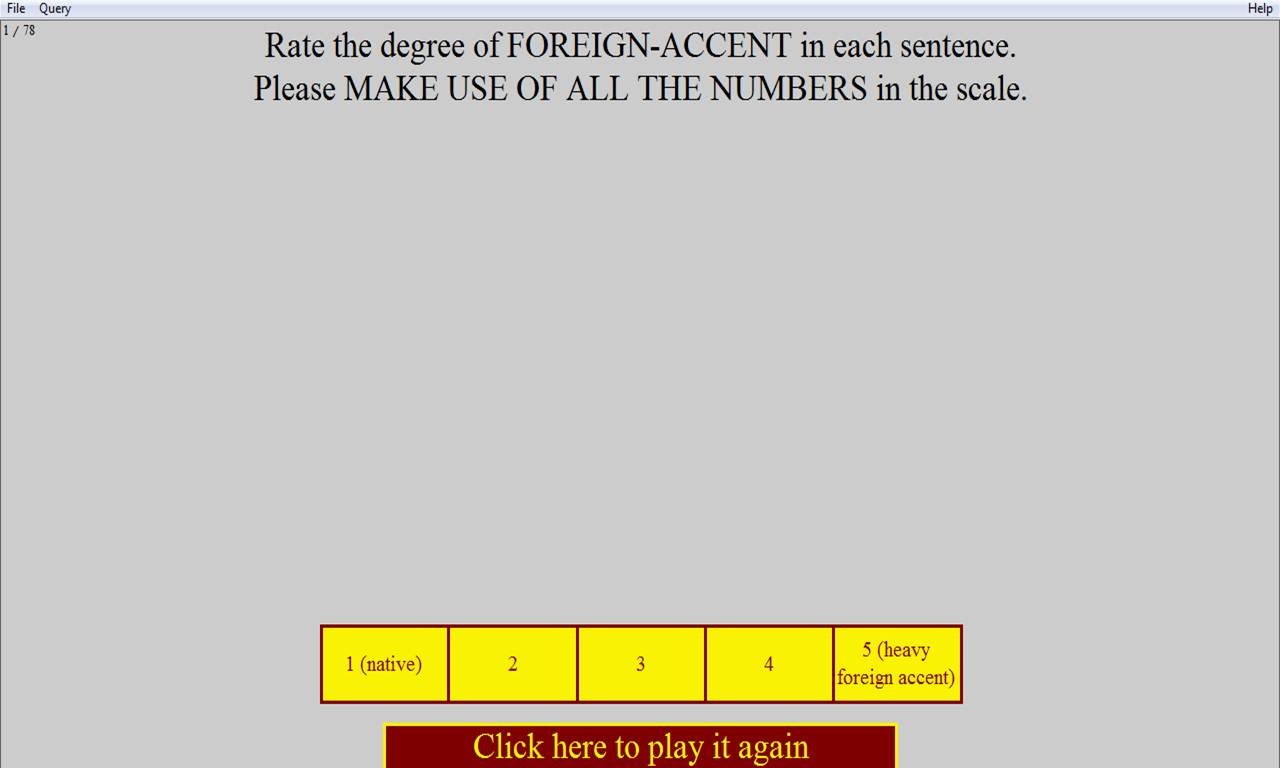
\includegraphics[width=5.028in,height=2.7362in,width=\textwidth]{avello-img1.jpg}
 
\end{styleStandard}

\begin{styleStandard}
\textit{Figure 1: Initial Praat screen for the rating task.}
\end{styleStandard}

\begin{styleStandard}
A 9-point scale has been most commonly used in FA studies, since participants usually differ greatly in proficiency level, as well as in AOL and/or L2 exposure. However, a 5-point scale was deemed more appropriate for the data in the present study, taking into account the smaller degree of variability in our oral samples (NNSs with a similar age, AOL, L2 exposure and proficiency level).
\end{styleStandard}

\begin{styleStandard}
Listeners were instructed to focus on pronunciation and rate the degree of FA they perceived in the speech samples as produced by the NNSs and the NSs by making use of the whole scale. Each stimulus was repeated twice for a total of 54 test trials per listener (8 NNSs x 3 data collection times x 2 repetitions + 3 NSs x 2 repetitions), resulting in a total of 702 ratings (54 trials x 13 listeners). Each listener heard the stimuli in a different randomized order. Listeners could replay each trial twice before providing their answer. After rating a stimulus, they had to click on a “next” button to listen to the following stimulus. If the NLs made a mistake when rating a stimulus, they could click on an error button to listen to it again and change their answer (an answer could be changed only once). Listeners were presented with 16 practice trials (8 samples x 2 repetitions) before the test trials. During the test trials, there was the possibility of a pause after a block of 18 trials.
\end{styleStandard}

\begin{listWWNumxxiileveli}
\item 
\begin{stylelsSectioni}
Results
\end{stylelsSectioni}

\end{listWWNumxxiileveli}
\begin{styleStandard}
Preliminary analyses were conducted to assess both intra-rater and inter-rater consistency in the NLs’ ratings by means of Pearson correlations, which yielded both high intra-rater and inter-rater consistency coefficients. 
\end{styleStandard}

\begin{styleStandard}
Regarding intra-rater reliability, there was a strong correlation in the listener-based FA ratings assigned at each of the two rating repetitions (\textit{r} = .71, \textit{p} = .007), indicating that each listener’s first and second repetition ratings were strongly correlated; that is, each listener assigned similar ratings to the same stimulus at both the first and second repetitions.
\end{styleStandard}

\begin{styleStandard}
Similarly, strong correlations were found in the stimulus-based FA ratings assigned by the 13 listeners in all pair-wise combinations, with \textit{r} coefficients ranging between .74 and .98 (in all cases \textit{p} {\textless} .05), which indicates a high degree of agreement among listeners.
\end{styleStandard}

\begin{styleStandard}
Table 1 and Figure 2 show the FA ratings assigned by the NLs to the baseline data provided by the NSs (T0) and to the NNSs through time (T1, T2 and T3). As expected, the ratings for the NSs were very close to 1 (\textit{M} = 1.06), indicating that the listeners identified the English NSs and rated them accordingly. In contrast, the ratings assigned to the NNSs’ were considerably outside the range of the NSs’ ratings across all testing times. 
\end{styleStandard}

\begin{flushleft}
\tablehead{}
\begin{supertabular}{m{0.7545598in}m{0.7538598in}m{0.7545598in}m{0.7538598in}m{0.7594598in}m{0.7545598in}m{0.7552598in}}
\hline
\bfseries Group &
\bfseries Time &
\bfseries \textit{n} &
\bfseries Minimum &
\bfseries Maximum &
\bfseries Mean &
\bfseries \textit{SD}\\\hline
\mdseries NS &
\mdseries T0 &
\mdseries 3 &
\mdseries 1.00 &
\mdseries 1.19 &
\mdseries 1.06 &
\mdseries .11\\\hline
\mdseries NNS &
\mdseries T1 &
\mdseries 8 &
\mdseries 2.58 &
\mdseries 4.58 &
\mdseries 3.19 &
\mdseries .68\\
\mdseries ~ &
\mdseries T2 &
\mdseries 8 &
\mdseries 2.62 &
\mdseries 4.23 &
\mdseries 3.47 &
\mdseries .49\\
\mdseries ~ &
\mdseries T3 &
\mdseries 8 &
\mdseries 3.04 &
\mdseries 3.81 &
\mdseries 3.40 &
\mdseries .31\\\hline
\end{supertabular}
\end{flushleft}
\begin{styleStandard}
\textit{Table 1: Summary for FA ratings as assigned by the NLs (1 = native,} 5 = heavy foreign accent).
\end{styleStandard}

\begin{styleStandard}
  [Warning: Image ignored] % Unhandled or unsupported graphics:
%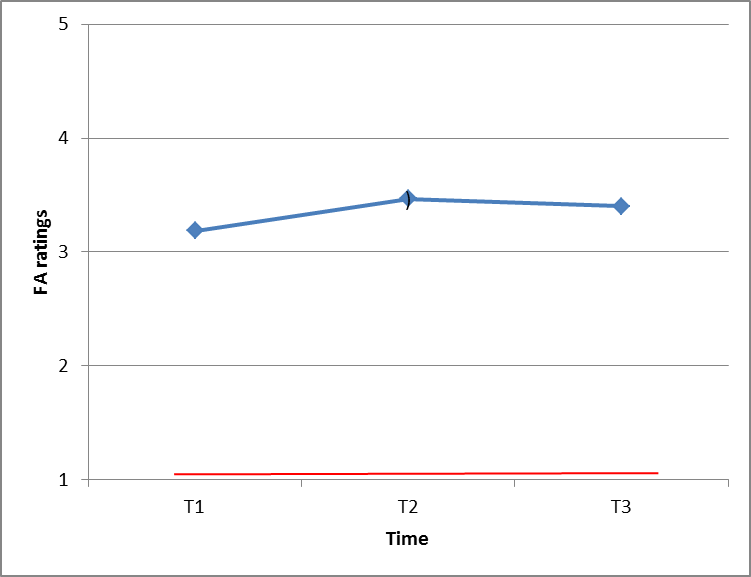
\includegraphics[width=4.4957in,height=3.4543in,width=\textwidth]{avello-img2.png}
 
\end{styleStandard}

\begin{styleStandard}
\textit{Figure 2: Mean FA ratings for the NSs (represented by the horizontal line) and the NNSs at T1 (at the beginning of the academic year), T2 (after an 80-hour FI period prior to SA) and T3 (upon return from a 3-month SA).}
\end{styleStandard}

\begin{styleStandard}
An increase in FA ratings can be observed between T1 (\textit{M} = 3.19) and T2 (\textit{M} = 3.47), signaling no positive effect of FI on the NNSs’ degree of FA. This is followed by a slight decrease in FA ratings between T2 (\textit{M} = 3.47) and T3 (\textit{M} = 3.40), which seems to suggest a positive trend of improvement in the NNSs’ degree of FA during the SA period. A one-way repeated measures ANOVA was conducted with the FA ratings as dependent variable and time as within-subjects factor in order to assess the effect of the FI and SA learning contexts on the L2 learners’ pronunciation development as measured by the FA ratings. This analysis yielded a non-significant effect of time on the FA ratings (Wilks’ Lambda = .64, \textit{F}(2, 6) = 1.69, \textit{p} = .26, \textit{$\eta $}\textit{\textsuperscript{2 }}= .36), indicating that the slight decrease observed in the FA ratings as a result of SA failed to reach significance.\footnote{ Results pooled across all listeners are presented, as the same results pattern was observed in the exchange students and English teachers.}
\end{styleStandard}

\begin{styleStandard}
Indeed, as illustrated in Table 1 and Figure 2, the L2 learners’ FA ratings remained similar through time. Independent samples \textit{t}{}-tests showed significant differences between the ratings assigned by the listeners to the NSs’ and to the NNSs’ at T1 (\textit{t}(9) = $-$5.21, \textit{p} \ = .001, \textit{$\eta $}\textit{\textsuperscript{2 }}= \ .75), T2 (\textit{t}(9) = $-$8.17, \textit{p} {\textless} .001, \textit{$\eta $}\textit{\textsuperscript{2 }}= .88), and T3 (\textit{t}(9) = $-$12.42, \textit{p} {\textless} .001, \textit{$\eta $}\textit{\textsuperscript{2 }}= .94). However, no significant differences were found between the three testing times for NNSs, which indicates the lack of development toward NS patterns in terms of degree of FA. Taken together, these results yield no evidence of significant improvement in FA ratings during SA, although they seem to signal a positive trend of development toward less accented speech as a result of SA (as opposed to FI). This suggests that SA might have had some impact on reducing the NNSs’ degree of accentedness, even though statistically non-significant.
\end{styleStandard}

\begin{listWWNumxxiileveli}
\item 
\begin{stylelsSectioni}
Discussion
\end{stylelsSectioni}

\end{listWWNumxxiileveli}
\begin{styleStandard}
These results contrast with the findings reported in most studies assessing the effect of SA on L2 acquisition. As noted in §2.2, SA has been generally found to have a clear positive impact on L2 linguistic development, with results providing evidence of substantial SA gains in lexical development (Collentine 2004; Llanes \& Muñoz 2009), writing (Sasaki 2004; Pérez-Vidal \& Juan-Garau 2011) and listening (Allen \& Herron 2003; Llanes \& Muñoz 2009). SA has been found to be particularly beneficial for the development of L2 oral skills, such as overall oral proficiency, enhanced accuracy and complexity, and most notably fluency (Brecht et al. 1995; Segalowitz \& Freed 2004; Valls-Ferrer 2011). This is in line with the general assumption that oral production is one of the areas that can be expected to improve the most during SA, as it is assumed to be one of the most practiced skills while abroad and to specially benefit from the massive exposure to L2 input that SA offers.
\end{styleStandard}

\begin{styleStandard}
However, these results are consistent with the scant existing research analyzing SA gains in L2 pronunciation, which has yielded inconclusive evidence regarding the effects of SA on this dimension. Whereas some studies have reported a positive effect of SA, for instance, on the production of consonantal segments (Díaz-Campos 2004; 2006; Mora 2008; Sanz et al. 2013), and rhythm metrics (Valls-Ferrer 2011), other studies have failed to find substantial SA gains in vowel production (Simões 1996; Avello 2010a; Pérez-Vidal et al. 2011), and in the production of both vowel and consonantal contrasts (Højen 2003). Avello (2010b) found that lack of improvement in vowel contrast production following SA did not prevent however considerable gains in FA scores. Conversely, results in Avello et al. (2012) showed significant improvement in phonetic measures of error rate scores during SA, whereas no significant improvement was found in FA ratings. 
\end{styleStandard}

\begin{styleStandard}
The lack of a stronger impact of SA on the FA ratings attributed to L2 learners in the present study may be related to the length of the SA program. LoS is one of the SA program features identified by Pérez-Vidal and Juan-Garau (2011) as influencing SA outcomes, since it determines amount of exposure to L2 input. LoS would thus be the SA equivalent to LOR, which is the variable that has traditionally been used as an index for amount of exposure to L2 input in FA studies analyzing the acquisition of L2 speech within long-term, naturalistic immersion contexts. 
\end{styleStandard}

\begin{styleStandard}
In his study addressing FA changes during SA by a group of L1 Danish undergraduate learners of English, Højen (2003) reported significant improvement in his participants’ FA scores after their experience abroad. However, the participants in his study presented considerable variation in terms of LoS in the SA context. The mean LoS was 7.1 months (range = 3-11 months), which is considerably longer than the 3-month stay experienced by the learners in the present study. When analyzing these individual differences, Højen found a strong positive correlation between LoS and gains in FA scores (\textit{r} = .61, \textit{p} {\textless} .05). The learners who showed less improvement during SA were those with stays of only 3 to 4 months, which is in line with the results of the present study, whereas the greatest SA gains were obtained by the learners who stayed abroad up to 11 months. Højen interpreted these results as signaling the importance of LoS for SA gains in FA scores to accrue.
\end{styleStandard}

\begin{styleStandard}
As indicated in §2.1 above, findings regarding the role of LOR on degree of FA in long-term immersion contexts have been mixed, with some studies reporting an effect of LOR on FA ratings while other studies have failed to do so. The impact of LOR seems to be influenced by L2 learners’ age and stage of L2 learning. LOR seems to have an effect on L2 pronunciation for early learners, but not for late or adult learners (Flege 1988). It has been claimed that most L2 phonological learning for late or adult L2 learners would take place within the first year of massive exposure in the L2 context. Pronunciation would then fossilize, resisting further changes after this initial period of gains (Selinker 1972; Flege 1988; Scovel 1988; Flege \& Fletcher 1992). More inexperienced late L2 learners (those at an early stage of L2 learning) could thus benefit from additional L2 exposure, whereas more experienced late L2 learners (those with higher proficiency) would be unlikely to benefit from further L2 exposure.
\end{styleStandard}

\begin{styleStandard}
The results reported in the present study could be interpreted in the light of these general findings for LOR effects. Although the NNSs in this study had been learning English since childhood in FI settings at their AH institutions, opportunities for out-of-class exposure to conversational English input are rather limited in Spain. The SA experience allowed them to live in an English-speaking country and to have access to massive and authentic L2 English input. However, as stated above, a 3-month LoS might be too short to observe significant improvement in these learners’ FA ratings. Considering that there seemed to be a tendency toward a decrease in accentedness during SA, it is possible that the NNSs’ degree of FA would have continued to gradually decrease with an increase in LoS up to, for example, the average 7.1 months or 11 months at which significant improvement in FA scores was reported by Højen (2003).
\end{styleStandard}

\begin{styleStandard}
Improvement in FA ratings seems to be further influenced by other factors, such as the actual amount and quality of the L2 input learners receive. According to Piske et al. (2001: 197), the inconclusive findings of research on LOR effects can also be partly due to the fact that “LOR only provides a rough index of overall L2 experience”. Following this line of thought, Højen (2003) created a composite measure which weighted LoS by self-reported English-language input while abroad, and found that the correlation between this composite measure and gains in FA scores (\textit{r} = .81, \textit{p} {\textless} .001) was stronger than the correlation between LoS alone and gains in FA scores as reported above. He interpreted this finding as an indication of the importance of having access to a substantial amount of high-quality L2 native input to improve FA scores, in line with previous findings (Flege \& Liu 2001).
\end{styleStandard}

\begin{styleStandard}
The learners in the present study reported a relatively high degree of contact with English NSs (an average of 3.6 on a 5-point scale, where 1 = ‘never’, 5 = ‘very often’), but they also reported a higher degree of contact with other NNSs of English (an average of 4.5 on the same scale). Since these learners were Erasmus students, it is very likely that they were in contact with other Erasmus students from a variety of non-English speaking countries. Exposure to this poorer, foreign-accented L2 input could have thus contributed to the lack of significant improvement in their FA ratings. In terms of accommodation, only one learner reported sharing an apartment with English NSs, whereas the rest reported staying in a single room at a residence hall. The fact that this was the preferred type of accommodation for the learners in this study might also have had some bearing on the lack of significant FA gains, as this type of accommodation is more likely to limit opportunities for interaction with NSs as compared with other options, such as sharing a room or apartment with NSs or staying with a native family.
\end{styleStandard}

\begin{styleStandard}
Another factor that has been found to influence FA gains is learners’ patterns of L1 and L2 use during immersion in the L2 context. Results reported in previous research suggest that more frequent use of the L1 (which would entail less frequent use of the L2) is associated with higher degree of FA (Flege et al. 1997; Piske et al. 2001). As is normally the case with Erasmus programs, the learners in the present study traveled to their SA destination in small groups and reported spending some time with the other students from their AH university (an average of 1.5 on a 3-point scale, where 1 = ‘most time’, 3 = ‘little’). The learners further reported a rather high degree of contact with their families back home while abroad by means of a scale from ‘a’ to ‘e’ (‘a’ = ‘more than once a day’ and ‘e’ = ‘none’). Learners reported mostly ‘b’ (‘a few times a week’), indicating frequent contact, whereas none reported ‘d’ or ‘e’. These patterns of rather frequent L1 use could also have prevented the learners from obtaining greater gains in their FA ratings.
\end{styleStandard}

\begin{styleStandard}
The lack of greater changes in the learners’ FA ratings could also be related to the way in which listeners process speech samples and how this influences their FA ratings. Listeners seem to assess speech samples for overall degree of FA holistically (Magen 1998). This means that they pay attention to different speech features both at the segmental level (phonemic and subphonemic substitutions, insertions, deletions) and suprasegmental level (stress, pitch range, rhythm, speaking rate, connected speech phenomena, overall prosody, or intonation), and that different listeners may also weigh these features of speech differently for different L2 learners and proficiency levels. Some studies have reported a positive effect of a short SA program not exceeding 3 months on learners’ segmental production (Díaz-Campos 2004; 2006; Mora 2008; Sanz et al. 2013). However, a 3-month SA program might not be long enough to trigger similar gains in other areas of pronunciation involving prosodic features of speech, which have also been found to considerably bear on the perception of FA (Anderson-Hsieh, Johnson \& Kohler 1992; Munro \& Derwing, 1999).
\end{styleStandard}

\begin{styleStandard}
Another factor which could have influenced the outcome of the FA ratings is the rather homogeneous composition of the learner group in terms of L2 proficiency level. Although there were differences in pronunciation between the learners, they all shared a similar L1 background and L2 English language level (B2 or upper-intermediate). This could have made the rating task rather difficult for the listeners, who had to discriminate subtle FA changes between learners and across testing time. It is probably easier for listeners to rate speech samples from a pool of learners showing a wider range of proficiency levels, from low to advanced. This has typically been the case in the FA literature examining long-term immersion contexts, where differences in FA scores arise as a result of considerable inter-subject variation in terms of L2 proficiency, which in turn can be attributed to differences in AOL, as well as to other variables such as L2 exposure, L1/L2 use, etc. (see §2.1). It is also possible that the use of a scale wider than the 5-point scale used in the present study would have better captured the slight changes in pronunciation that the learners might have experienced. \ 
\end{styleStandard}

\begin{listWWNumxxiileveli}
\item 
\begin{stylelsSectioni}
Conclusion
\end{stylelsSectioni}

\end{listWWNumxxiileveli}
\begin{styleStandard}
To sum up, results in the present study showed no improvement in the NNSs’ FA ratings as a result of FI and suggested, in contrast, a positive trend of development toward a decrease in FA following SA, although this decrease was not significant and the NNSs’ FA ratings remained significantly different from the NSs’ FA ratings through time. This outcome is in line with the mixed results that have been reported in the scarce research that has assessed the effect of SA as compared with FI on L2 pronunciation. Given the observed trend of development during SA, maybe an increased LoS could have resulted in continued gradual improvement leading to significant gains in the NNSs’ FA ratings, as is suggested in previous research (Højen 2003). Since general findings from research on L2 speech production suggest that most progress in pronunciation takes place during the first year of immersion in an L2 context, more studies are needed focusing on the effects of LoS on pronunciation outcomes for L2 learners with different proficiency levels. 
\end{styleStandard}

\begin{styleStandard}
Considering the holistic way in which listeners provide FA ratings, and the fact that different listeners may focus on different aspects of L2 speech, it is also possible that the FA ratings in the present study failed to reflect some gains that could have accrued in some specific features of the learners’ L2 pronunciation. Such changes could have been captured by fine-grained phonetic or acoustic analyses, or could have been reflected in the FA ratings by means of the use of a scale with a wider range. Previous research has found that the relation between FA ratings and specific aspects of pronunciation is not always a straightforward one. For example, Avello et al. (2012) found significant SA gains in phonetic error rate scores, but not in FA scores. Conversely, in Riney \& Flege (1998), gains in global FA ratings did not coincide with improvement in segmental production regarding liquid identifiability and accuracy. The authors noted that it “appears not to be the case that improvement in global accent necessarily proceeds in parallel with improvement in any particular smaller components of pronunciation, such as segmental identifiability and accuracy” (p. 237). In this sense, in order to gain better insight into the types of changes that can be expected in L2 pronunciation as a result of SA, more research is needed with a multiple-measures approach that combines subjective FA scores as well as more objective acoustic and phonetic analyses that include acoustic measures and error rate scores.
\end{styleStandard}

\begin{stylelsSectioni}
Acknowledgements
\end{stylelsSectioni}


\begin{styleStandard}
This research was funded by grant FFI2010-21483-C02-01 awarded by the Spanish Government to the SALA project, and by grants BES-2008-010037 and EEBB-I-12-04294 awarded by the Spanish Government to the author within the FPI doctoral research program.
\end{styleStandard}

\begin{stylelsSectioni}
References
\end{stylelsSectioni}


\begin{styleStandard}
Allen, Heather W. \& Herron, Carol. 2003. A mixed-methodology investigation of the linguistic and affective outcomes of summer study abroad. \textit{Foreign Language Annals} 36(3). 370–385.
\end{styleStandard}


\begin{styleStandard}
Anderson-Hsieh, Janet \& Johnson, Ruth \& Kohler, Kenneth. 1992. The relationship between native speaker judgments of nonnative pronunciation and deviance in segmentals, prosody, and syllable structure. \textit{Language Learning} 42(4). 529–555.
\end{styleStandard}


\begin{styleStandard}
Avello, Pilar. 2010a. The effect of study abroad on Catalan/Spanish bilinguals’ production of English /i: - [26A?]/ and /æ - [28C?]/ contrasting pairs. (Paper presented at the 6th International Conference on Language Acquisition - CIAL, Universitat de Barcelona, Spain.) 
\end{styleStandard}


\begin{styleStandard}
Avello, Pilar. 2010b. Study abroad and foreign accent: The production of /i: - [26A?]/ and /æ - [28C?]/ by Catalan/Spanish bilinguals. (Paper presented at the 20th International Conference of the European Second Language Association - Eurosla, University of Modena and Reggio Emilia, Italy.)
\end{styleStandard}


\begin{styleStandard}
Avello, Pilar. \& Mora, Joan C. \& Pérez-Vidal, Carmen. 2012. Perception of FA by non-native listeners in a study abroad context. \textit{Research in Language} 10(1). 63–78.
\end{styleStandard}


\begin{styleStandard}
Barron, Anne. 2006. Learning to say {\textquotesingle}you{\textquotesingle} in German: The acquisition of sociolinguistic competence in a study abroad context. In Margaret A. DuFon \& Eton E. Churchill (eds.), \textit{Language learners in study abroad contexts}, 59–90. Clevedon, UK: Multilingual Matters.
\end{styleStandard}


\begin{styleStandard}
Best, Catherine T. \& Tyler, Michael D. 2007. Nonnative and second-language speech perception. In Ocke-Schwen Bohn \& Murray J. Munro (eds.), \textit{Language experience in second language speech learning: In honour of James Emil Flege}, 13–34. Amsterdam: Benjamins.
\end{styleStandard}


\begin{styleStandard}
Boersma, Paul \& Weenink, David. 2008. \textit{Praat: Doing phonetics by computer}. http://www.fon.hum.uva.nl/praat/
\end{styleStandard}


\begin{styleStandard}
Bongaerts, Theo \& Planken, Brigitte \& Schils, Erik. 1995. Can late starters attain native accent in a foreign language? A test of the critical period hypothesis. In David Singleton \& Zsolt Lengyel (eds.), \textit{The age factor in second language acquisition: A critical look at the critical period hypothesis}, 30–50. Clevedon, UK: Multilingual Matters.
\end{styleStandard}


\begin{styleStandard}
Bongaerts, Theo \& van Summeren, Chantal \& Planken, Brigitte \& Schils, Erik. 1997. Age and ultimate attainment in the pronunciation of a foreign language. \textit{Studies in Second Language Acquisition} 19(4). 447–465.
\end{styleStandard}


\begin{styleStandard}
Brecht, Richard \& Davidson, Dan \& Ginsberg, Ralph 1995. Predictors of foreign language gain during study abroad. In Barbara Freed (ed.), \textit{Second language acquisition in a study abroad context}, 37–66. Amsterdam: Benjamins.
\end{styleStandard}


\begin{styleStandard}
Coleman, James A. 1998. Language learning and study abroad: The European perspective. \textit{Frontiers}: \textit{The Interdisciplinary Journal of Study Abroad} 4. 167–203.
\end{styleStandard}


\begin{styleStandard}
Collentine, Joseph. 2004. The effects of learning contexts on morphosyntactic and lexical development. \textit{Studies in Second Language Acquisition} 26(2). 227–248.
\end{styleStandard}


\begin{styleStandard}
DeKeyser, Robert. 2007. Study abroad as foreign language practice. In Robert DeKeyser (ed.), \textit{Practice in a second language: Perspectives from applied linguistics and cognitive psychology}, 208–226. Cambridge: Cambridge University Press
\end{styleStandard}


\begin{styleStandard}
del Río, Carmen. 2013. \textit{Perceived foreign accent and comprehensibility in the oral production of adolescent learners of English: study abroad vs. at home learning contexts}. Barcelona: Universidad Pompeu Fabra. (Doctoral dissertation.)
\end{styleStandard}


\begin{styleStandard}
Derwing, Tracey M. \& Munro, Murray J. 1997. Accent, intelligibility, and comprehensibility: Evidence from four L1s. \textit{Studies in Second Language Acquisition} 20(1). 1–16.
\end{styleStandard}


\begin{styleStandard}
Derwing, Tracey M. \& Munro, Murray J. 2013. The development of L2 oral language skills in two L1 Groups: A 7-year study. \textit{Language Learning} 63(2). 163–185.
\end{styleStandard}


\begin{styleStandard}
Díaz-Campos, Manuel 2004. Context of learning in the acquisition of Spanish second language phonology. \textit{Studies in Second Language Acquisition} 26. 249–273. 
\end{styleStandard}


\begin{styleStandard}
Díaz-Campos, Manuel 2006. The effect of style in second language phonology: An analysis of segmental acquisition in study abroad and regular-classroom students. In Carol A. Klee \& Timothy L. Face (eds.), \textit{Selected proceedings of the 7th conference on the acquisition of Spanish and Portuguese as first and second Languages}, 26–39. Sommerville, MA: Cascadilla Proceedings Project. 
\end{styleStandard}


\begin{styleStandard}
DuFon, Margaret A. \& Churchill, Eton E. (eds.). 2006. \textit{Language learners in study abroad contexts}. Clevedon, UK: Multilingual Matters.
\end{styleStandard}


\begin{styleStandard}
Flege, James E. 1988. Factors affecting degree of perceived foreign accent in English sentences. \textit{Journal of the Acoustical Society of America} 84(1). 70–79.
\end{styleStandard}


\begin{styleStandard}
Flege, James E. 1995. Second language speech learning theory, findings, and problems. In Winifred Strange (ed.), \textit{Speech perception and linguistic experience: Issues in cross-language research}, 233–277. Timonium, MD: York Press.
\end{styleStandard}


\begin{styleStandard}
Flege, James \ E. \& Fletcher, Kathryn L. 1992. Talker and listener effects on degree of perceived foreign accent\textit{. Journal of the Acoustical Society of America} 91(1). 370–389.
\end{styleStandard}


\begin{styleStandard}
Flege, James E. \& Frieda, Elaina M. \& Nozawa, Takeshi. 1997. Amount of native-language (L1) use affects the pronunciation of an L2. \textit{Journal of Phonetics} 25(2). 169–186.
\end{styleStandard}


\begin{styleStandard}
Flege, James E. \& Liu, Serena. 2001. The effect of experience on adults{\textquotesingle} acquisition of a second language. \textit{Studies in Second Language Acquisition} 23(4). 527-–52.
\end{styleStandard}


\begin{styleStandard}
Flege, James \ E. \& Munro, Murray J. \& Mackay, Ian R. A. 1995. Effects of age of second-language learning on the production of English consonants. \textit{Speech Communication} 16(1). 1–26.
\end{styleStandard}


\begin{styleStandard}
Freed, Barbara. (ed.). 1995a. \textit{Second language acquisition in a study abroad context}. Amsterdam: Benjamins.
\end{styleStandard}


\begin{styleStandard}
Freed, Barbara. 1995b. What makes us think that students who study abroad become fluent? In Freed, B. (ed.), \textit{Second language acquisition in a study abroad context}, 123–148. Amsterdam: Benjamins.
\end{styleStandard}


\begin{styleStandard}
Freed, Barbara. \& Dewey, Dan P. \& Segalowitz, Norman \& Halter, Randall. 2004. The language contact profile. \textit{Studies in Second Language Acquisition} 26(2). 349–356.
\end{styleStandard}


\begin{styleStandard}
Howard, Martin. 2005. Second language acquisition in a study abroad context: A comparative investigation of the effects of study abroad and foreign language instruction on the L2 learner{\textquotesingle}s grammatical development. In Alex Housen \& Michel Pierrard (eds.), \textit{Investigations in instructed second language acquisition}, 495–530. Berlin: Mouton de Gruyter. 
\end{styleStandard}


\begin{styleStandard}
Højen, Anders Damgren. 2003. \textit{Second-language speech perception and production in adult learners before and after short-term immersion}. Aarhus: University of Aarhus. (Doctoral dissertation.)
\end{styleStandard}


\begin{styleStandard}
IPA. 1999. \textit{Handbook of the International Phonetic Association}. Cambridge: Cambridge University Press.
\end{styleStandard}


\begin{styleStandard}
Kinginger, Celeste. 2009. \textit{Language learning and study abroad}. Basingstoke: Palgrave Macmillan.
\end{styleStandard}


\begin{styleStandard}
Lafford, Barbara. 1995. Getting into, through and out of a survival situation: A comparison of communicative strategies used by students studying Spanish abroad and {\textquotesingle}at home{\textquotesingle}. In Barbara Freed (ed.), \textit{Second language acquisition in a study abroad context}, 97–122. Amsterdam: Benjamins.
\end{styleStandard}


\begin{styleStandard}
Lenneberg, Eric H. 1967. \textit{Biological foundations of language}. New York: John Wiley \& Sons.
\end{styleStandard}


\begin{styleStandard}
Long, Michael. 1990. Maturational constraints on language development. \textit{Studies in Second Language Acquisition} 12(3). 251–285.
\end{styleStandard}


\begin{styleStandard}
Llanes, Àngels. \& Muñoz, Carmen. 2009. A short stay abroad: Does it make a difference? \textit{System} 37(3). 353–365.
\end{styleStandard}


\begin{styleStandard}
Magen, Harriet S. 1998. The perception of foreign-accented speech. \textit{Journal of Phonetics} 26(4). 381–400.
\end{styleStandard}


\begin{styleStandard}
Meador, Diane \& Flege, James E. \& Mackay, Ian R. A. 2000. Factors affecting the recognition of words in a second language. \textit{Bilingualism: Language and Cognition} 3(1). 55–67.
\end{styleStandard}


\begin{styleStandard}
Mora, Joan C. 2008. Learning context effects on the acquisition of a second language phonology. In Carmen Pérez-Vidal \& Maria Juan-Garau \& Aurora Bel (eds.), \textit{A portrait of the young in the new multilingual Spain}, 241–263. Clevendon, UK: Multilingual Matters. 
\end{styleStandard}


\begin{styleStandard}
Munro, Murray J. 1998. The effects of noise on the intelligibility of foreign-accented speech. \textit{Studies in Second Language Acquisition} 20. 139–154.
\end{styleStandard}


\begin{styleStandard}
Munro, Murray J. \& Derwing, Tracey M. 1995. Foreign accent, comprehensibility, and intelligibility in the speech of second language learners. \textit{Language Learning} 45(1). 73–97. 
\end{styleStandard}


\begin{styleStandard}
Munro, Murray J. \& Derwing, Tracey M. 1998. The effects of speaking rate on listener evaluations of native and foreign-accented speech. \textit{Language Learning} 48(2). 159–182.
\end{styleStandard}


\begin{styleStandard}
Munro, Murray J. \& Derwing, Tracey M. 1999. Foreign accent, comprehensibility, and intelligibility in the speech of second language learners. \textit{Language Learning} 49. 285–310.
\end{styleStandard}


\begin{styleStandard}
Pérez-Vidal, Carmen \& Juan-Garau, Maria. 2011. The effect of context and input conditions on oral and written development: A study abroad perspective. \textit{International Review of Applied Linguistics in Language Teaching} 49(2). 157–185.
\end{styleStandard}


\begin{styleStandard}
Pérez-Vidal, Carmen \& Juan-Garau, Maria \& Mora, Joan C. 2011. The effects of formal instruction and study abroad contexts on foreign language development: The SALA project. In Cristina Sanz \& Ronald P. Leow (eds.), \textit{Implicit and explicit conditions, Processes and knowledge in SLA and bilingualism}, 115–138. Washington D. C.: Georgetown University Press.
\end{styleStandard}


\begin{styleStandard}
Piske, Thorsten \& MacKay, Ian R. A. \& Flege, James E. 2001. Factors affecting degree of foreign accent in an L2: A review. \textit{Journal of Phonetics} 29(2). 191–215.
\end{styleStandard}


\begin{styleStandard}
Riney, Timothy \& Flege, James E. 1998. Changes over time in global foreign accent and liquid identifiability and accuracy. \textit{Studies in Second Language Acquisition} 20. 213–243.
\end{styleStandard}


\begin{styleStandard}
Sanz, Cristina \& Morales-Front, Alfonso \& Nagle, Charlie \& Moorman, Colleen 2013. Learning without attention: Improvements in pronunciation in a 6 week study abroad program. (Paper presented at the Residence Abroad, Social Networks and Second Language Learning Congress, University of Southampton, UK.)
\end{styleStandard}


\begin{styleStandard}
Sasaki, Miyuki. 2004. A multiple-data analysis of the 3.5-year development of EFL student writers. \textit{Language Learning} 54(3). 525–582.
\end{styleStandard}


\begin{styleStandard}
Schneider, Edgar W. \& Burridge, Kate \& Kortmann, BBernd \& Mesthrie, Rajend \& Upton, Clive (eds.). 2004. \textit{A Handbook of varieties of English. Volume 1: Phonology}. Berlin: Mouton de Gruyter.
\end{styleStandard}


\begin{styleStandard}
Scovel, Thomas. 1988. \textit{A time to speak. A psycholinguistic inquiry into the critical period for human speech}. Cambridge, MA: Newbury House Publishers.
\end{styleStandard}


\begin{styleStandard}
Segalowitz, Norman \& Freed, Barbara. 2004. Context, contact and cognition in oral fluency acquisition: Learning Spanish in at home and study abroad contexts. \textit{Studies in Second Language Acquisition} 26(2). 173–199.
\end{styleStandard}


\begin{styleStandard}
Selinker, Larry. 1972. Interlanguage. \textit{International Review of Applied Linguistics in Language Teaching} 10(3). 209–231.
\end{styleStandard}


\begin{styleStandard}
Simões, Antonio R. M. 1996. Phonetics in second language acquisition: An acoustic study of fluency in adult learners of Spanish. \textit{Hispania} 79(1). 87–95.
\end{styleStandard}


\begin{styleStandard}
Valls-Ferrer, Margalida. 2011. \textit{The development of oral fluency and rhythm during a study abroad period. }Barcelona: Universidad Pompeu Fabra. (Doctoral dissertation.) 
\end{styleStandard}

\end{document}
